\documentclass{article}
\usepackage[utf8]{inputenc}
\usepackage{graphicx}
\usepackage[super,negative]{nth}
\usepackage{fancyhdr}
\usepackage{float}

\renewcommand{\thefigure}{\arabic{section}.\arabic{figure}}

\begin{document}
	\begin{titlepage}
		
		\centering
		\vspace*{0.7 cm}
		
\includegraphics[scale = 0.7]{images/PolimiLogo.png}\\[1 cm]
		\textsc{\large Dipartimento di Elettronica, Informazione e Bioingegneria}\\[2 cm]
		
		\rule{\linewidth}{0.2 mm} \\[0.5 cm]
		{\huge \bfseries Requirement Analysis and Specification Document (RASD)}\\
		\rule{\linewidth}{0.2 mm} \\[1.5 cm]
		
		\textsc{\Large SafeStreets}\\[0.5 cm]
		\textsc{\large - v1.0 -}\\[1 cm]
		
		\begin{minipage}{\textwidth}
			\begin{flushleft} \large
				\emph{Authors:}\\
				\textbf{Quacquarelli}, Sebastiano \hfill 945071 \\
				\textbf{Ricchiuti}, Simone \hfill 945613  \\
				\textbf{Sala}, Nicolò \hfill matricola3 \\[2 cm]
			\end{flushleft}
		\end{minipage}\\[2 cm]
		
		{\large November \nth{10} , 2019}\\[2 cm]
		
	\end{titlepage}
	
	\pagenumbering{roman}
	\tableofcontents
	
	\newpage
	\pagenumbering{arabic}
	\setcounter{page}{1}
	
	\section{Introduction}
	\subsection{Purpose}
	
	SafeStreets is an application that allows its users to notify possible traffic violations to authorities, which can evaluate them and eventually generate traffic tickets.\\
	SafeStreets can also collect information about incidents from authorities and combine them with information about violations to let users do data-mining and to show them statistics.\\
	Finally, SafeStreets can combine the retrieved information to suggest to authorities some possible solutions for particularly unsafe areas.\\
	
	\subsection{Scope}
	A user can report a violation using SafeStreets application
	
	\subsection{Definitions, Acronyms, Abbreviations}
	\subsection{Revision history}
	\subsection{Reference Documents}
	\subsection{Document Structure}
	
	\newpage
	\section{Overall description}
	\subsection{Product perspective}
	In Figure 2.1 is given a visual representation about shared phenomena and domain model. 
	\begin{figure}[ht]
		\centering
		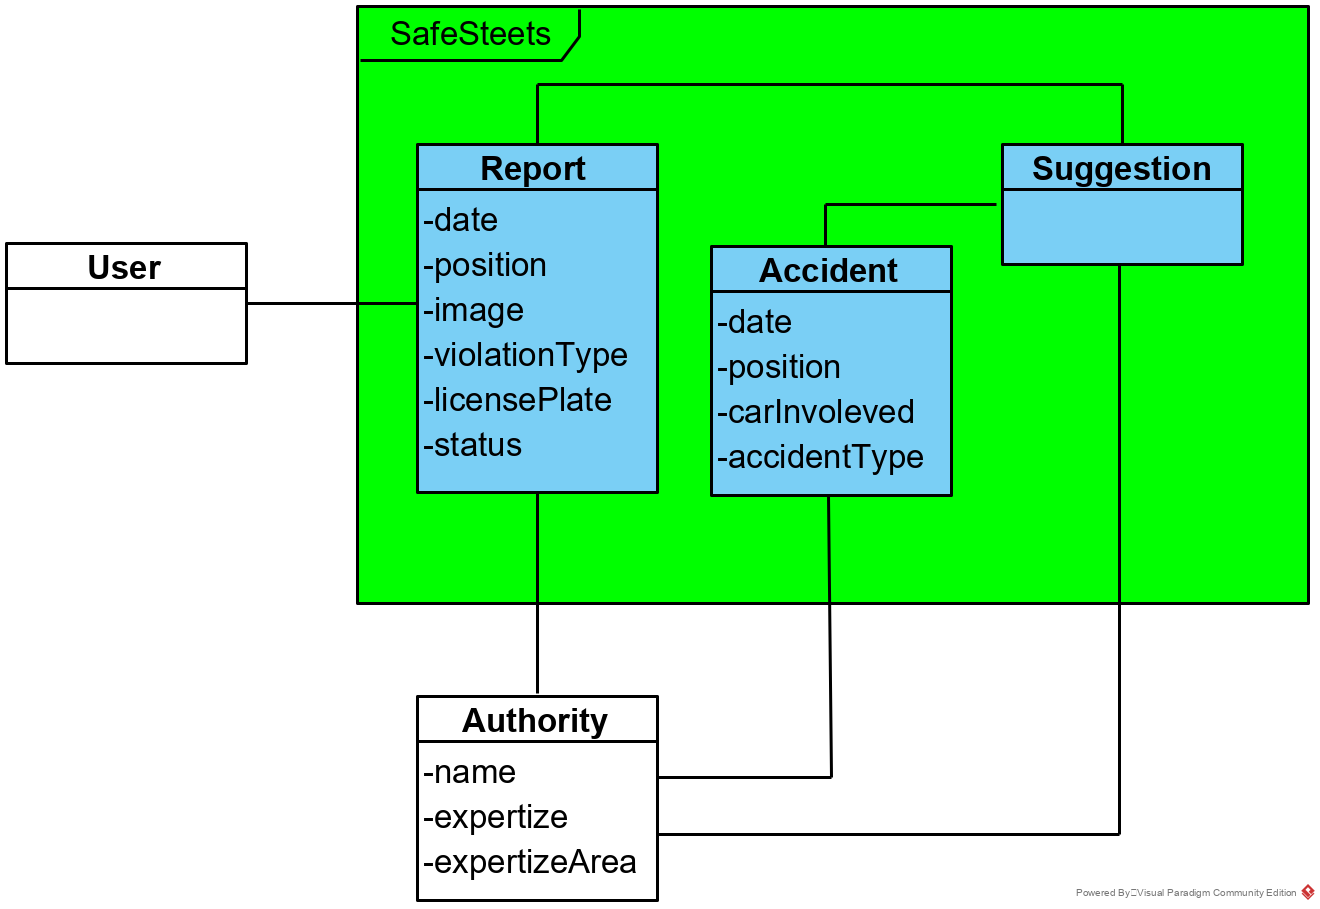
\includegraphics {diagrams/domain_model.png}
		\caption[Domain Model]{Domain Model}
		\label{fig:domain_model}
	\end{figure}
	
	The users can interact with SafeStreets system through a mobile application and reporting some traffic violations.
	SafeStreets does not collect any data about users, so they are represented as a black box. The interaction between user and SafeStreets is established only through 
	a report, which will be published in SafeStreets system.\\\\
	An authority registered on SafeStreets can be noticed about traffic violations reported in its own operative area and eventually evaluate if report is correct or not. Moreover, an authority can report to SafeStreets any information about accidents in order to identify unsafe areas and suggest possible interventions.\\\\
	To understand the main events in SafeStreets system, some statechart diagrams are represented in figures below. \\\\
	\clearpage
	Figure \ref{fig:statechart_userReporting} explains how SafeStreets works when a user try to report traffic violation.
	
	\begin{figure}[H]
		\centering
		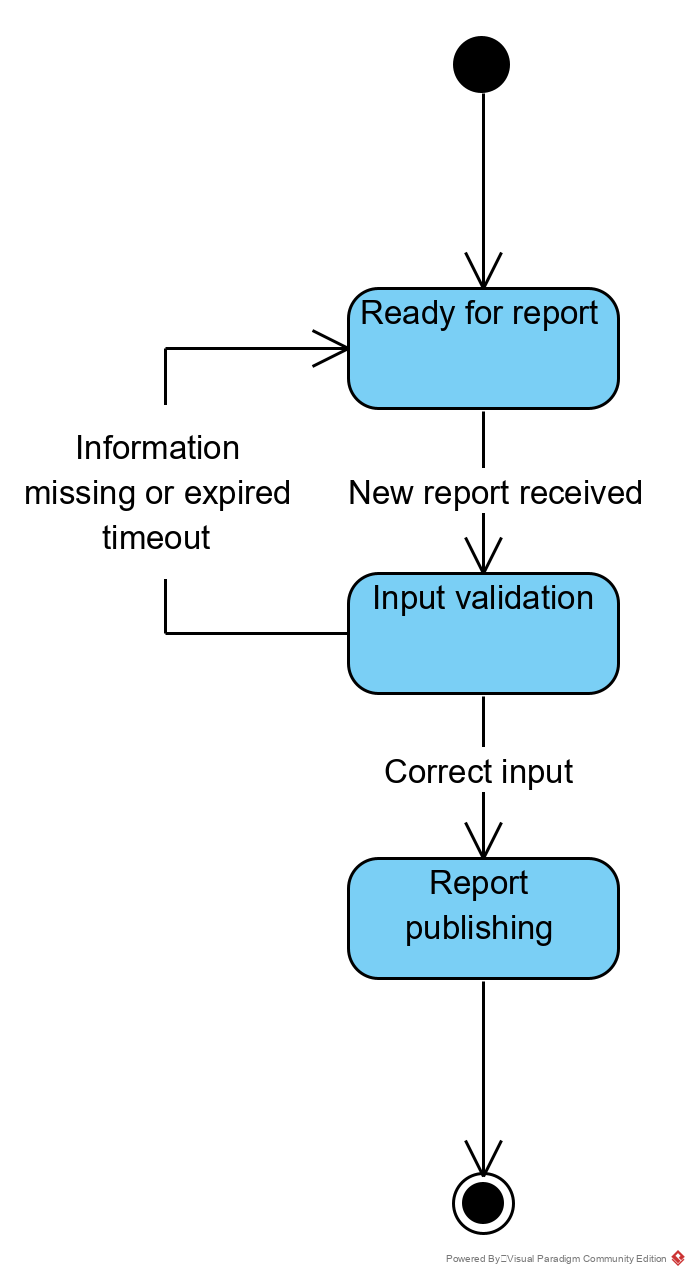
\includegraphics[width=0.5\textwidth]{diagrams/statechart_UserSS.png}
		\caption[Statechart Diagram1]{Statechart Diagram about user reporting.}
		\label{fig:statechart_userReporting}
	\end{figure}
	
	The core of application is based on users' reports: the more reports there are, the more the system can provide information about areas in a municipality. Before publishing, SafeStreets does an input valuation: it doesn't have means to check if a report could actually be a traffic violations, but uses them to show areas from which reports are from.
	
	\begin{figure}[H]
		\centering
		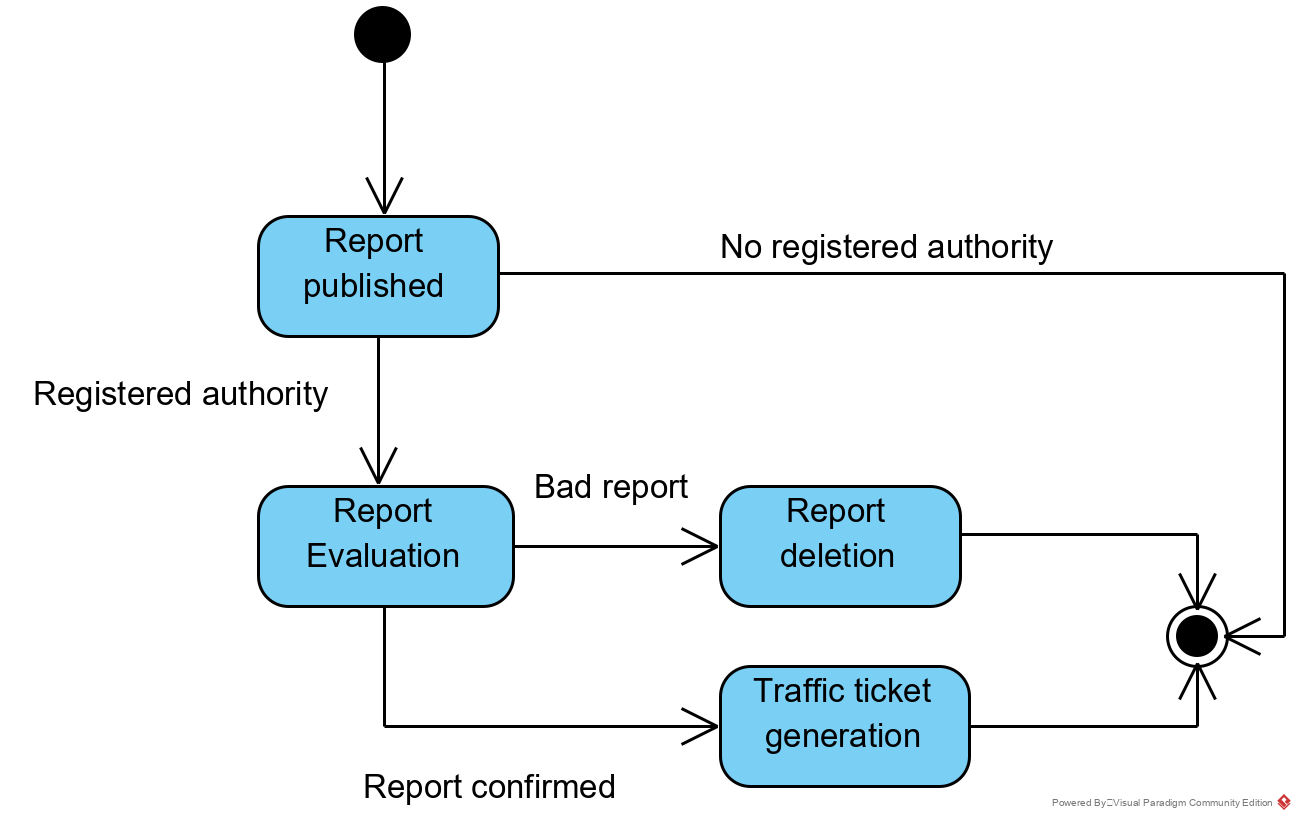
\includegraphics {diagrams/statechart_AuthoritySS.png}
		\caption[Statechart Diagram2]{Statechart Diagram about SafeStreets' suggestions for an authority.}
		\label{fig:statechart_SuggestionsForAuthority}
	\end{figure}
	
	Figure \ref{fig:statechart_SuggestionsForAuthority} shows how SafeStreets operate with an authority.\\
	Authorities could eventually have some information about accidents in their operative zone and can decide to share them with SafeStreets.\\
	SafeStreets collect these data and try to cross them with reports about traffic violations: if for an area there are frequent violations or accidents, SafeStreets suggests possible interventions.
	
	\clearpage	   
	
	\subsection{Product functions}
	In the following section all the main product functions are defined. Basically the reporting and data-mining functions are considered the basic ones, then the other functions are advanced ones offered by SafeStreets thanks to the collaboration with authorities. Thus, if authorities, in a defined area, are not sharing information with SafeStreets, these advanced functions are not available in that area.
	\subsubsection{Violation reporting}
	This is the core function of SafeStreets. The aim of this function is to give to the user the possibility to report a traffic violation. The system allows the user to use this function without a previous login. The user is asked to complete his reporting action defining the following fields:\\
	- Picture representing the violation;\\
	- Type of violation.\\
	Other important information such as position, date and time of the violation are taken by GPS and metadata associated to the report.\\
	In particular, to take the requested picture, the user is allowed only to use the in-app dedicated camera tool in order to prevent users from reporting past violation uploading old pictures.\\ The picture is approved by the app if and only if the license plate is correctly recognized by the dedicated algorithm, otherwise, the app will ask to the user to make it again. If, after some attempts, SafeStreets' app warns that is still not possible to recognize the license plate, the user is asked to insert it manually. \\The type of violation is selectable only by the ones offered by SafeStreets.\\ The user is asked also to complete these two requests in a defined interval of time in order to guarantee the consistency of the report offered to SafeStreets.\\
	When a violation is correctly filled in, it is sent to the system which will publish it and will make it visible to users.\\
	Each violation is automatically sent to a competent authority, if available, and then will be managed by it.
	
	\subsubsection{Data-mining}
	This function allows the user to analyze SafeStreets' data in order to mine some information, for example, by highlighting the streets (or the areas) with the highest frequency of violations, or the vehicles that commit the most violations. The kind of information requested can be filtered by user in order to restrict the research area. \\
	
	\subsubsection{Interactive suggestions}
	This function is strictly related to the collaboration between SafeStreet's data, offered by users' reports, and authorities, which can enrich the database including information about the accidents that occur. \\SafeStreet can cross all these information and it can also identify potentially unsafe areas suggesting possible interventions to authorities. \\
	In a more detailed way, this function, analyzing data and making a comparison between them and some defined limit parameters, can automatically detect possible standard-defined improvements, create suggestions useful to reduce violations and accidents.
	
	\subsubsection{Traffic tickets}
	This function is specially addressed to authorities. SafeStreets ensuring the integrity of its data allows authorities to use them to generate traffic tickets. \\
	The authority can define the final judgement about a report received, modifying its status.\\
	If a report is judged consistent (so its state has been updated) SafeStreets knows that a traffic tickets has been generated from it, otherwise the report is cancelled.\\
	Furthermore, SafeStreets can analyze issued tickets (consistent reports) and it can create statistics for example about the most egregious offenders, or the effectiveness of the SafeStreets initiative by looking for rends in the issuing of tickets.
	
	
	\subsection{User characteristics}
	The actors of the application are the following:
	\begin{itemize}
		\item User: a person that is using SafeStreet's app. He is a "guest" because he is not logged in, so no specific information about him are given. He can actively use the first two basic functions so he can make a violation reporting or data-mining.
		\item Authority: special kind of user. It is allowed to use the user's functions but also including additional privileges on them such as to visualize more detailed information about reports. In particular, it is a registered identity that is responsible to manage its competent reports. Authority can send to SafeStreets information about accidents of its area of competence and can use SafeStreet's statistics to identify the most egregious offenders.
		A kind of authority is the Police, that can use reports to make traffic tickets validating them.
	\end{itemize}
	
	\subsection{Assumptions, dependencies and constraints}
	
	
	\section{Specific requirements}
	\subsection{External Interfaces Requirements}
	\subsubsection{User Interfaces}
	\subsubsection{Hardware Interfaces}
	\subsubsection{Software Interfaces}
	\subsubsection{Communication Interfaces}
	\subsection{Functional Requirements}
	\subsection{Performance Requirements}
	\subsection{Design Constraints}
	\subsubsection{Standards compliance}
	\subsubsection{Hardware limitations}
	\subsubsection{Any other constraint}
	\subsection{Software System Attributes}
	\subsubsection{Reliability}
	\subsubsection{Availability}
	\subsubsection{Security}
	\subsubsection{Maintainability}
	\subsubsection{Portability}
	
	\section{Formal analysis using Alloy}
	
	\section{Effort spent}
	
	\section{References}
	
	
\end{document}
